\documentclass[12pt,twoside,a4paper]{article}
\usepackage[utf8]{inputenc} \usepackage[T1]{fontenc} \usepackage{graphicx}
\begin{document}

Subtraktion von binären Zahlen

Drei Schritte zu Subtraktion:

Das Einerkomplement
Das Zweierkomplement
Die Subtraktion von Dualzahlen

Einerkomplement

Was ist das Komplement von Dualzahlen? Man bildet das sogenannte Einerkomplement, indem man jede Zahl durch ihr Gegenteil ersetzt, also die 0 durch die 1 und die 1 durch die 0.

01011010 wird zu 10100101
11101101 wird zu 00010010

\paragraph{Das Zweierkomplement}

Das Zweierkomplement entspricht dem Einerkomplement, nur wird zusätzlich noch 00000001 addiert.

01011010 wird im Einerkomplement zu 10100101 im Zweierkomplement zu 10100110
11101101 wird im Einerkomplement zu 00010010 im Zweierkomplement zu 00010011

\paragraph{Konvertierung von Festkommazahlen Dez zu Bin}

10,2 \\
\\

Vorkommastelle
10 = 1010

Nachkommastelle\\
\emph{0,2} * 2 = 0,4 + 0 \emph{MSB} \\ 
0,4 * 2 = 0,8 + 0\\
0,8 * 2 = 0,6 + 1\\
0,6 * 2 = \emph{0,2} + 1 \emph{LSB} \\ 

Sobald es sich wiederholt kann aufgehört werden.\\
0, 2 = 0,0011\\
10,2 \^= 1010,00110011 \approx 0,19921875
\\
\Longrightarrow Eine Abweichung von  -0,00078125
\\
\paragraph{Konvertierung von Fließkommazahlen Dez zu Bin}
18,4_{10}


\item {18_{10}  \^= 10010_{2}} 
\item {0,4_{10} \^= 0,011_{2}}
\end






\paragraph{Die Subtraktion von Dualzahlen}

Der Satz lautet: Die Subtraktion von 2 Zahlen erfolgt durch die Addition des Zweierkomplementes. Als konkretes Beispiel nehmen wir dazu die Rechnung 14-9=5.

9 ist im Dualsystem 00001001.
Das Einerkomplement zu 00001001 ist 11110110.
Das Zweierkomplement 11110111.
Dies addieren wir nun zu 14 also 00001110.

   00001110 
  +11110111 
   ========
   00000101

Auch hier wäre die richtige Zahl eigentlich 00000101 Übertrag 1, da wir den Übertrag jedoch nicht speichern können, bleiben wir bei 00000101 was ja der Dezimalzahl 5 entspricht.

\paragraph{Little-/Bigendian}
\begin{figure}[ht!]
\centering
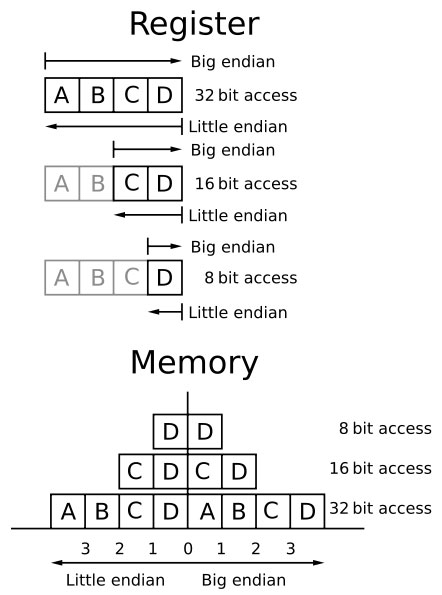
\includegraphics[width=90mm]{big-endian_und_little-endian.jpg}
\caption{A simple caption \label{overflow}}
\end{figure}

\paragraph{Assemblerbefehle}
AREA MyCommonBlock, COMMON, ALIGN = 10 ; Read-Write-Data
MyCommonBlock bezeichnet die Anfangsadresse des Speicherblocks
COMMON: vom Linker mit Nullen initialisierter Speicherbereich
Alignment mit 2^{10} erzeugt eine Blockgrenze bzw. –anfang mit n * 1024

mov r0, #0x21
Lade #0x21 in Register R0:
R0
00000021

\subparagraph{Angabe negativer Konstanten}
mov r1, #-10



\end{document}
